\chapter{Implementation}
This chapter focuses on the implementation details of the container runtime 
and the benchmark tool. 

Section \ref{ch:implementation/runtime} dives deeply into the 
system call interface of the Linux kernel that enables the creation and execution 
of isolated workloads.

Section \ref{ch:implementation/benchmark} presents the implementation of the benchmarks
and the tool that manages them. 

\label{ch:implementation}
\section{Runtime}
\label{ch:implementation/runtime}
The runtime is divided into two parts - a library and an executable.
Section \ref{ch:implementation/runtime/library} contains information about how 
the library was implemented as well as a qualitative description of its security characteristics.

Section \ref{ch:implementation/runtime/executable} shifts the focus towards the runtime executable,
also referred to as a \textit{container shim}, and its responsibilities.
\subsection{Library}
\label{ch:implementation/runtime/library}
The \verb|clone()| system call is the runtime's primary method of isolating a process.
This system call creates a new execution context and allows the caller to configure it 
through a bit mask. In essence, this bit mask defines the noninterference boundary between 
the new execution context, its parent, and all other processes on the system. If the bit mask is 0, 
the clone system call is equivalent to a simple \verb|fork()|. The runtime utilises this 
system call for two purposes - to spawn the container process in a new set of namespaces and to 
create a pollable process file descriptor for it. 
\begin{lstlisting}[style=c-code-snippets, label={code:implementation/namespaces/clone}, caption={Container instantiation within the runtime using clone3}]
static inline pid_t clone3(struct clone_args *args, size_t args_size)
{
    return (pid_t) syscall(SYS_clone3, args, args_size);
}

static int container_entrypoint(void *arg)
{
    struct conty_container *cc = (struct conty_container *) arg;
    /* Configure container within new namespace set */
    /* At the end, call execve to load the user-defined binary */
}

int conty_container_spawn(struct conty_container *cc)
{
    struct clone_args args = {
        // cc->cc_ns_new contains
        // CLONE_NEWIPC | CLONE_NEWPID | CLONE_NEWUSER | CLONE_NEWNS | CLONE_NEWUTS | CLONE_NEWNET
        .flags = cc->cc_ns_new | CLONE_PIDFD;
        .pidfd = (__u64)(uintptr_t) &cc->cc_pollfd,
    };

    cc->cc_pid = clone3(&args, CLONE_ARGS_SIZE_VER2);
    if (cc->cc_pid == 0) 
        /* Within container */
        _exit(container_entrypoint(cc));
    else 
        /* Within runtime */
}
\end{lstlisting}
    
Achieving the former is trivial. The kernel exposes a flag for every namespace type.
These flags are simply ORed together and passed into the system call. 
Internally, the kernel allocates a new namespace proxy and all of its namespaces 
in a system-wide slab cache and attaches it as a pointer to the new task structure.
Whenever a process attempts to operate on a namespaced resource, the kernel follows its reference to the 
proxy, and the resources' reference to the namespace. If the resource is managed by the same namespace 
that the process is a part of, then the respective operation is permitted.
Code snippet \ref{code:fundamentals/namespaces/process} shows an example of how clone is used 
within the runtime implementation. The namespaces are parsed from the configuration file and 
aggregated into a bit mask \verb|cc_ns_new|. The runtime then calls out to the \verb|clone3()| system call
with the namespace mask set, as well as a pointer to a pollable file descriptor for the 
container that should be populated by the kernel - \verb|cc_pollfd|. 

Spawning a process in a new set of namespaces is not enough to provide a secure runtime environment.
As a matter of fact, the container's runtime environment after \verb|clone()| is insecure and unusable.
The runtime must configure the environment depending on the namespaces that were created.

If the runtime creates a container process with the \verb|CLONE_NEWUSER| flag set, i.e in a new user namespace,
the kernel initialises the container's security context to an unprivileged state by setting its 
user and group identifiers to the overflow value, also known as the \enquote{nobody} user.
This user has the least privileges on the system, making the new user namespace particularly unuseful. 
Even if the namespace manages security-sensitive resources, such as network devices and mount points,
the container process is considered unprivileged to access them. For this reason, the container runtime 
has the responsibility of remapping the invalid identifiers to valid user identifiers. 
It is particularly important to note that the remapped identifiers must refer to users within 
the root user namespace, i.e on the host. The remapping is done by writing a range of 
identifiers to the files \verb|/proc/[pid]/uid_map| and \verb|/proc/[pid]/gid_map| where \verb|pid|
refers to the process identifier of the container.
These files consist of multiple entries separated by newline characters. 
An entry is represented by three integers - $c$, $h$ and $a$. 
The kernel maps the half-open range of identifiers $[c, c+a)$ to $[h, h+a)$ where 
$c$ denotes the starting identifier in the container's user namepace and $h$ denotes 
the starting identifier in the root user namespace.
\begin{lstlisting}[label={code:implementation/namespaces/user-example}, style=bash, caption={Example of an identifier mapping}]
$ cat /proc/self/uid_map
0 1000 50
\end{lstlisting}
Consider the example in code snippet \ref{code:implementation/namespaces/user-example}. The 
runtime has mapped the root user in the container's user namespace to the user with identifier 1000 
on the host. Similarly, user 1 in the container is mapped to user 1001 on the host. The same logic 
applies to all users up to 49 and 1049 inside the container and on the host, respectively. 
If a malicious attacker gains access to a container and manages to break out of its user namespace, 
protecting the host system depends on the identifier mapping. In the example above, the 
attacker will still be unprivileged on the host, provided that users $(1000, 1049)$ are unprivileged.
If, however, the runtime writes a mapping
\begin{equation}
    c = h = 0;  a = 1, \label{eq:implementation/root-mapping}
\end{equation}
a container escape proves critical.
The mapping in (\ref{eq:implementation/root-mapping}) is the default one for containers created by the Docker engine, necessitating
additional configurations to enable rootless containers.
The identifier mappings of a container also have an impact on its noninterference boundary with 
other containers. If the runtime maps the same user identifer on the host to the root user inside the user namespaces of two different containers, an 
attacker that escapes from one container will be able to enter the user namespace of the other. Upon entering,
the attacker will have root privileges. Therefore, for a truly secure environment, two invariants must hold - 
mapped identifier ranges must not overlap across different containers, and a privileged user on the host must 
not be mapped to a user inside a container. The kernel imposes several restrictions to user-space for 
writing to the map files. First, the kernel prohibits more than a single write to such a file. 
That is, the runtime can write only once to that file. Furthermore, at least one line must be 
written to the file. An attacker that subsequently attempts to manipulate the mappings would not 
be able to. Secondly, the writing process must have the \verb|CAP_SETUID| and 
\verb|CAP_SETGID| capabilities in the root user namespace, or otherwise it can 
write only a single entry into the file. Deciding which identifier mappings to write is a function 
of a container engine, not the runtime. The runtime simply reads the identifier mappings
from a configuration file like the one defined in code snippet \ref{code:oci-config.json}, buffers 
them in memory and dumps them to the respective map files from within the container process.
This is the very first thing that the container process does to ensure that subsequent operations
are properly authorised by the kernel. 

Creating a process with the \verb|CLONE_NEWNS| flag puts it in a new mount namespace that 
inherits a copy of the parent's mount points. This includes the parent's root mount (at \verb|/|),
which contains various \enquote{submounts} such as the pseudo filesystems \verb|/proc| and \verb|/sys|,
the in-memory filesystem \verb|/dev| and all of its resident device nodes,
the POSIX message queue filesystem \verb|/dev/mqueue| and the POSIX shared-memory filesystem \verb|/dev/shm|.
The container runtime is responsible for setting up all of these filesystems inside the new mount namespace,
under the base directory of the container's dedicated root filesystem. Note that upon creation, the container's root filesystem is a simple directory, not a mount point. 
The runtime must convert it into a mount point so that it can replace the inherited root mount 
with a new one. Therefore, the runtime bind mounts the aforementioned directory onto itself, using 
the \verb|mount| system call. Recall from Section \ref{sections:fundamentals/namespaces/mount} 
that every mount point is associated with a propagation type. If the parent mount of the 
directory that holds the root filesystem has a shared propagation type, then bind mounting 
that directory inside the container will propagate the mount event downstream to the parent mount, 
causing the bind mount to appear in the set of mount points of the root mount namespace.
This is not desirable as it directly interferes with the host environment. For this reason, 
the container process first remounts the old root filesystem to have a private propagation type and 
only then performs the bind mount.
Note that setting the propagation type to \verb|MS_SLAVE| would also work, if the container 
wants to receive mount events from the host. This process is shown in code snippet \ref{code:implementation/namespaces/mount}.
The variable \verb|rfs->cro_dst| holds the absolute path to the container's root filesystem.
Afterwards, the runtime mounts the device filesystem as a \verb|tmpfs| instance and creates the
five device nodes listed in Table \ref{table:implementation/runtime/devices}.
Even though the container process is privileged in its user namespace and has the \verb|CAP_MKNOD|
capability set, trying to create the device nodes with the \verb|mknod()| system call fails with an
\verb|EPERM| error. Albeit an important resource inside a containerised environment, device nodes 
are not namespaced nor owned by a user namespace. 
Instead, the kernel resorts to authorising the operation with the user credentials in the initial 
root namespace, which will always fail in the context of a rootless container. For this reason,
the runtime falls back to bind mounting the devices from the host. 
Axiomatically, the noninterference boundary for these devices is nonexistent. 
\begin{lstlisting}[style=c-code-snippets, label={code:implementation/namespaces/mount}, caption={Remounting the original root filesystem to disable mount propagation events and bind mounting the container's root filesystem onto itself.}]
/* Error handling deliberately left out */
mount("", "/", "", MS_PRIVATE | MS_REC, NULL);
mount(rfs->cro_dst, rfs->cro_dst, "bind", MS_BIND | MS_REC, NULL);
mount("", rfs->cro_dst, "", MS_PRIVATE, NULL);
\end{lstlisting}

\begin{table}[h!]
    \centering
    \begin{tabular}{ |m{4cm}|m{20em}| }
        \hline
        Device & Description \\
        \hline
        \verb|null| & Data sink. Reads return EOF \\
        \hline 
        \verb|zero| & Data sink. Reads return null bytes \\
        \hline
        \verb|full| & Data sink/source emulating a full device. Reads return null bytes. Writes return \verb|ENOSPC| \\
        \hline
        \verb|random| & Random number generator gathering environmental noise from device drivers. Blocks until enough entropy is gathered. \\
        \hline
        \verb|urandom| & Random number generator gathering environmental noise from device drivers. Has nonblocking semantics \\
        \hline
    \end{tabular}
    \caption{Table of mounted device nodes within a container}
    \label{table:implementation/runtime/devices}
\end{table}

The same semantics apply when trying to mount a block device inside a 
rootless container. The block device must first be mounted within the root mount namespace, and 
then bind mounted from within the container's mount namespace. This, however, weakens the 
noninterference boundary. An attacker that escapes a container may interfere with other containers
by manipulating the device's mount point.

The \verb|proc| and \verb|sys| filesystems are mounted conditionally. The former presents information
about all processes on the system. If the runtime is instructed to create a container with 
its own isolated process identifier namespace, then it must mount a dedicated \verb|proc|
filesystem that replaces the old one. Otherwise, process information from the host environment 
will be leaked inside the container. Similarly, the \verb|sysfs| filesystem contains information 
about the system's network interfaces, routes, firewall rules and so on. If the container inherits 
this mount from the host, then networking information will be leaked. In addition, containerised 
processes that rely on the contents of that filesystem will not work properly. Therefore, 
the runtime replaces the old mount with a new one, provided that the user has requested a 
new network namespace. The kernel is instructed to disallow the creation of set-user-id programs,
executable files and device nodes within these filesystems. Write permissions are disabled 
for all users that are not mapped to the root user within the container's user namespace. 
After setting up all the mounts, the runtime pins the root filesystem onto the 
root directory entry, making all filesystem entries on the host inaccessible from within the container's mount namespace.
\begin{lstlisting}[style=c-code-snippets, label={code:implementation/namespaces/pivot}, caption={Swap the old root filesystem with a new one}]
/* Error handling deliberately left out */
int old_root = -EBADF, new_root = -EBADF;
new_root = openat(-EBADF, rfs->cro_dst, O_DIRECTORY | O_PATH | O_CLOEXEC | O_NOFOLLOW);
old_root = openat(-EBADF, "/", O_DIRECTORY | O_PATH | O_CLOEXEC | O_NOFOLLOW);
fchdir(new_root);
pivot_root(".", ".");
fchdir(old_root);
mount("", ".", "", MS_SLAVE | MS_REC, NULL);
umount2(".", MNT_DETACH);
fchdir(new_root);
\end{lstlisting}
This is achieved through the \verb|pivot_root| system call, which moves 
the old root mount to a location specified by the runtime and mounts the root filesystem at \verb|/|,
as shown in code snippet \ref{code:implementation/namespaces/pivot}.

The runtime overlays the old root mount on top of the new one, caching a file descriptor to the former 
before pivoting. It then switches its current directory by using the file descriptor and unmounts
the old root. 
Note that setting 
the old root filesystem's propagation type to \verb|MS_PRIVATE|, as shown on line 1 in code snippet 
\ref{code:implementation/namespaces/mount}, is a requirement for calling \verb|pivot_root|.
Otherwise, unmounting the old root filesystem may propagate downstream to the host, causing it to 
unmount as well.

Creating a process with the \verb|CLONE_NEWUTS| flag puts it in a new uts namespace that inherits 
a copy of the parent's system identifiers. The runtime reacts to this by setting the container's
hostname to a user-defined string present in the container's configuration file.

The runtime does not enforce a particular network configuration for a container. This is done 
by the container engine, or in our case, the benchmark tool. Hence, the runtime proceeds 
to call \verb|execve|. In turn, the kernel installs a fresh virtual address space 
for the process with the user program loaded. 
The runtime must ensure that all auxiliary file descriptors 
are closed before executing the program. Otherwise, these will be preserved in the file descriptor 
table of the process and leaked to the user program.
The most fault-tolerant way to do this is to open every file descriptor with the \verb|O_CLOEXEC|
flag. The kernel takes care of closing the file descriptors when \verb|execve| is called. 
Note that, for debugging purposes, the standard input-output streams are not closed and are 
therefore inherited. 

The runtime process and the container process need to synchronise with each other for two purposes.
First, the runtime allows external applications to plug into well-defined points in the 
lifecycle of a container and execute arbitrary binaries. 
\begin{table}[h!]
    \centering
    \begin{tabular}{ |m{4cm}|m{2cm}|m{2cm}|m{15em}| }
        \hline
        Event & Sender & Receiver & Event Description \\
        \hline
        \verb|EVENT_RT_CREATE| & Container & Runtime & Execute runtime creation hooks \\
        \hline
        \verb|EVENT_RT_CREATED| & Runtime & Container & Runtime creation hooks completed \\
        \hline 
        \verb|EVENT_CONT_CREATE| & Runtime & Container & Execute container creation hooks \\
        \hline 
        \verb|EVENT_CONT_CREATED| & Container & Runtime & Container creation hooks executed \\
        \hline
        \verb|EVENT_CONT_START| & Runtime & Container & Start user-defined binary \\
        \hline 
        \verb|EVENT_CONT_STARTED| & Container & Runtime & User-defined binary started \\
        \hline
    \end{tabular}
    \caption{Table of events exchanged by the runtime and the container}
    \label{table:implementation/runtime/socket-events}
\end{table}

For example, a set of hooks 
gets executed after the container pivots into its root filesystem but before it executes the user-defined 
binary. 
Hence, the container process needs to block and wait for a hook execution event from the 
runtime. Second, the runtime 
process must be able to receive error notifications from the container so that it knows 
when to reap the container and what to report to the user. The kernel provides a variety of 
inter-process communication mechanisms that can be grouped into two semantical categories - shared-memory 
and message passing. The runtime uses the latter. In particular, the container and runtime processes 
interact through a pair of full-duplex UNIX streaming sockets created with the \verb|socketpair()|
system call. The runtime and the container keep one end of the socket pair open 
and close the other end, respectively. Sockets have a natural point of synchronisation - if a 
process attempts to read any data from the socket, it blocks until data becomes available. Continuing the 
example above, when the container needs to execute a set of hooks before executing the user-defined 
binary, it reads from the socket, thereby blocking until the runtime process writes some data. Similarly, if the 
container process encounters an error, it writes a particular error message into the socket.
When the runtime reads from the socket, it will receive the error notification and perform 
the necessary cleanup operations. The complete summary of messages, as well as the sending and 
receiving parties are described in Table \ref{table:implementation/runtime/socket-events}.
The receiving party in each of the messages always blocks until the sender writes the message
to the underlying socket.

\subsection{Executable}
\label{ch:implementation/runtime/executable}
We now turn our focus onto the executable component, also referred to as a \textit{container shim}.
The shim sits between a container engine and a container runtime library. The shim is a process 
dedicated to managing a single container instance. It lives for the duration of the container
and takes on the responsibility of redirecting the container's standard input-output streams 
to log files that can be intercepted by the container engine. This functionality is beyond the scope of this work,
albeit trivial to implement. Instead, the container inherits the input-output streams of the shim. 
In addition, the shim is responsible for tracking 
and updating the container's state machine, as well as propagating signals sent by the container engine to the container. 
Both functionalities are implemented in a similar manner - 
by registering a file descriptor with an event loop and suspending the shim's execution until 
the file descriptor becomes active. The shim registers two file descriptors - a signal file 
descriptor that becomes active whenever the shim receives a signal from another process, and the 
container's pollable process file descriptor, which becomes active whenever the container process 
terminates. The creation of the latter is done via the \verb|clone()| system call and can be seen in code snippet \ref{code:implementation/namespaces/clone}.
The signal file descriptor is created via a dedicated system call - \verb|signalfd()| - 
that provides an alternative way of accepting signals besides registering a signal handler 
incapable of executing functions that are async-signal unsafe. The shim blocks all signals 
that aren't handled according to their default dispositions and registers the signals it would 
like to receive events on through a signal mask configured by calls to \verb|sigemptyset()|, 
\verb|sigaddset()| and \verb|sigprocmask()|. The file descriptor is subsequently registered 
with an event loop managed by the \verb|poll()| system call. This system call blocks 
the active thread until a file descriptor is ready. The system call populates a bit mask 
indicating what type of event occured. The shim is interested in a single event - \verb|POLLIN|,
which indicates that the file descriptor is readable. In the context of the container's file descriptor,
no data is available. This event simply indicates that the process has exited. In the context of the 
signal file descriptor, the shim can read a structure from it that holds the requested signal and 
afterwards propagate that signal to the container process.

The container shim provides a command-line interface to its users.
A user is required to specify the path to the container's configuration file, an eample 
of which is shown in code snippet \ref{code:oci-config.json}. In addition, the user must 
give the container a unique name. Optionally, the user may specify a timeout. The timeout is used 
by the shim to wait for the container to exit. If the timeout expires, the container is forcibly 
killed by the shim. The shim's command line interface is shown in code snippet \ref{code:implementation/runtime/conty-runner}.

\begin{lstlisting}[label={code:implementation/runtime/conty-runner}, style=bash, caption={Container shim command-line interface}]
$ conty-runner --help
Usage: conty-runner [OPTION...] NAME
conty-runner -- A program that runs containers

  -b, --bundle=PATH          Path to container bundle
  -t, --timeout[=NUMBER]     Time to wait for container to exit before killing
  -?, --help                 Give this help list
      --usage                Give a short usage message
  -V, --version              Print program version

Mandatory or optional arguments to long options are also mandatory or optional
for any corresponding short options.

Report bugs to htw-berlin.de.
\end{lstlisting}

\section{Benchmark}
The benchmark focuses on measuring network and filesystem latencies and throughput 
within and outside a container, respectively. The goal is to highlight the differences
in response time and efficiency (See Chapter \ref{ch:Experiment}).
Here, the tools used for measurement sampling and plot generation are discussed.
Additionally, implementation details surrounding the workloads are mentioned.

\label{ch:implementation/benchmark}
\subsection{Network workload}
The network workload introduced in Section \ref{ch:concept/benchmark/net-workload} 
was implemented with the help of the \verb|iperf3| program - a tool 
for performing network throughput and latency measurements for TCP and UDP.
This tool consists of two launch modes - server mode and client mode. 
The server can be launched by specifying the \verb|-s| option and the 
network address and port it should listen on, as shown in code snippet \ref{code:implementation/benchmark/network-workload}. 
By default, the server listens on port $5201$. 
\begin{lstlisting}[label={code:implementation/benchmark/network-workload}, style=bash, caption={Launching an iperf3 TCP server}]
$ iperf3 -s 192.168.8.2
\end{lstlisting}
The client is launched with the \verb|-c| option and the network address and port 
of the server it should connect to. In addition, the user can configure the 
number of parallel connections, the size of the buffers to be transmitted 
when interacting with the server, and the sampling duration. Furthermore,
the user can instruct the tool to output its measurement samples in JSON and to a file.
\begin{lstlisting}[label={code:implementation/benchmark/network-workload}, style=bash, caption={Launching an iperf3 TCP client that connects to an iperf3 server listening on 192.168.8.2 and writes performance samples gathered for 60 seconds from 5 parallel connections into a file}]
$ iperf3 --logfile out.iperf3 -J --parallel 5 --length 128k --time 60 -c 192.168.8.2
\end{lstlisting}
In the above example, the client writes a total of $60 \times N$ samples, i.e one sample per second, into the file where $N$ denotes the number of 
parallel connections. Each sample contains, amongst other things, the round-trip time measured in microseconds, the 
number of bits transfered per second, as well as the number of retransmits encountered during the time interval. 
To generate the plots, the file is preprocessed by a bash script that groups the aforementioned metrics
by connection and generates a folder with files storing the preprocessed data. Afterwards, the results are fed into the 
\verb|gnuplot| command-line program in order to generate the two-dimensinal plots shown in Section \ref{ch:experiment/network}.

\begin{figure}[H]
    \centering
    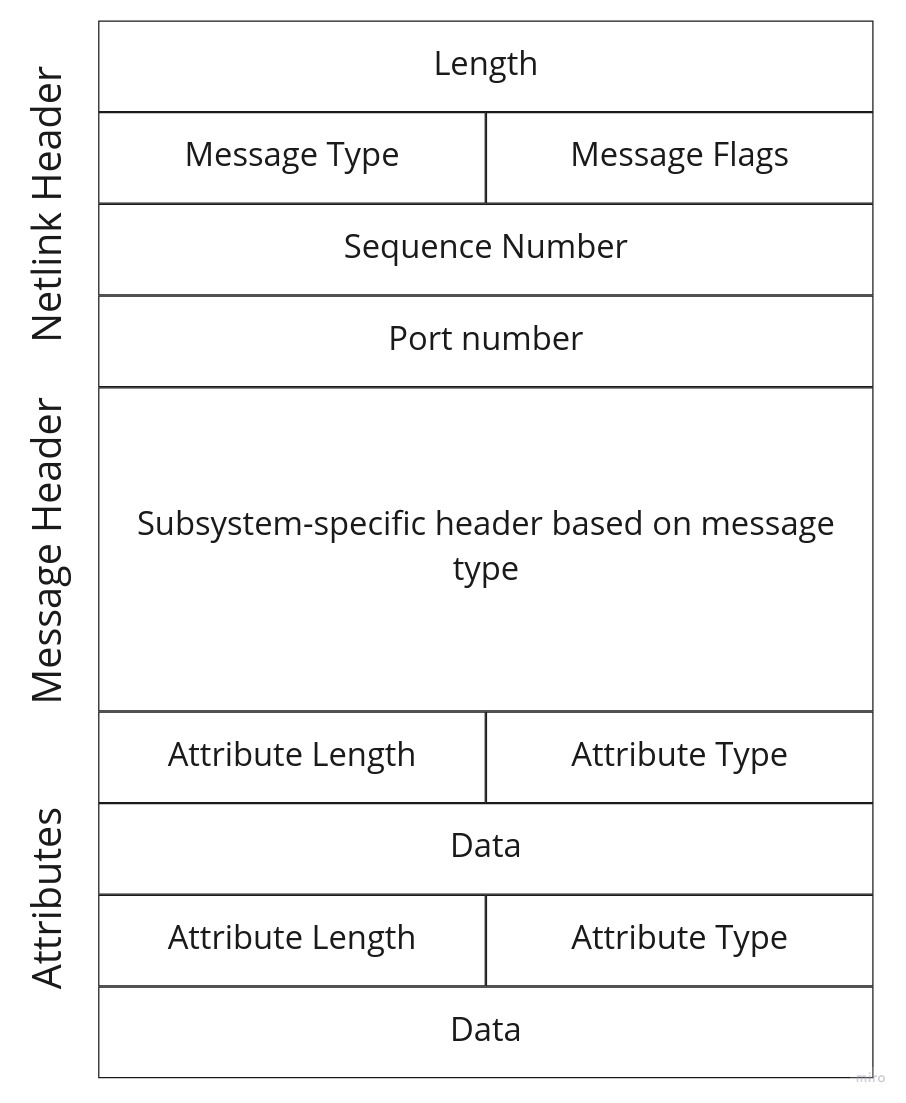
\includegraphics[width=0.5\textwidth]{images/implementation/netlink-message.jpg}
    \caption{Netlink message format}
    \label{images:implementation/netlink-message.jpg}
\end{figure}

The TCP client and server programs must run in two different containers in order to measure 
the isolation overhead of the network namespace abstraction. However, they cannot talk to each other 
unless properly configured. For this reason, a hook program was developed that sets up a virtual 
ethernet cable for both the client and server. The hook program is referenced within the 
client and server's container configuration files, under the \verb|on_runtime_create| hooks mentioned in Table \ref{table:concept/runtime/hooks}. 
The container runtime picks up the program and executes it when creating the containers.
In addition, the hook program sets up a bridge device (if it does not already exist) and attaches 
the virtual ethernet interface of the container to it. 
The interfaces are configured by interacting with the kernel through a datagram socket whose format 
is dictated by the netlink protocol.

The netlink protocol is based on messages that consist of a header and a payload.
Usually, the payload is further deconstructed into a subsystem-specific header that identifies 
a particular resource and a set of attributes that represent configurable properties of the resource.
The hook program specficially targets the routing subsystem, which manages resources like 
virtual network devices, their addresses and routing tables. The general message format 
is shown in Figure \ref{images:implementation/netlink-message.jpg}. Details pertaining to the protocol itself and the messages sent 
to setup the network infrastructure shown in Figure \ref{images:fundamentals/net-ns-veth-arch.jpg}
are described in Section \ref{ch:appendix/netlink-protocol}. 

For the sake of simplicity, the hook program was implemented in the Go programming language 
and utilised a library that hides the underlying details of the netlink protocol.

\begin{figure}[H]
    \centering
    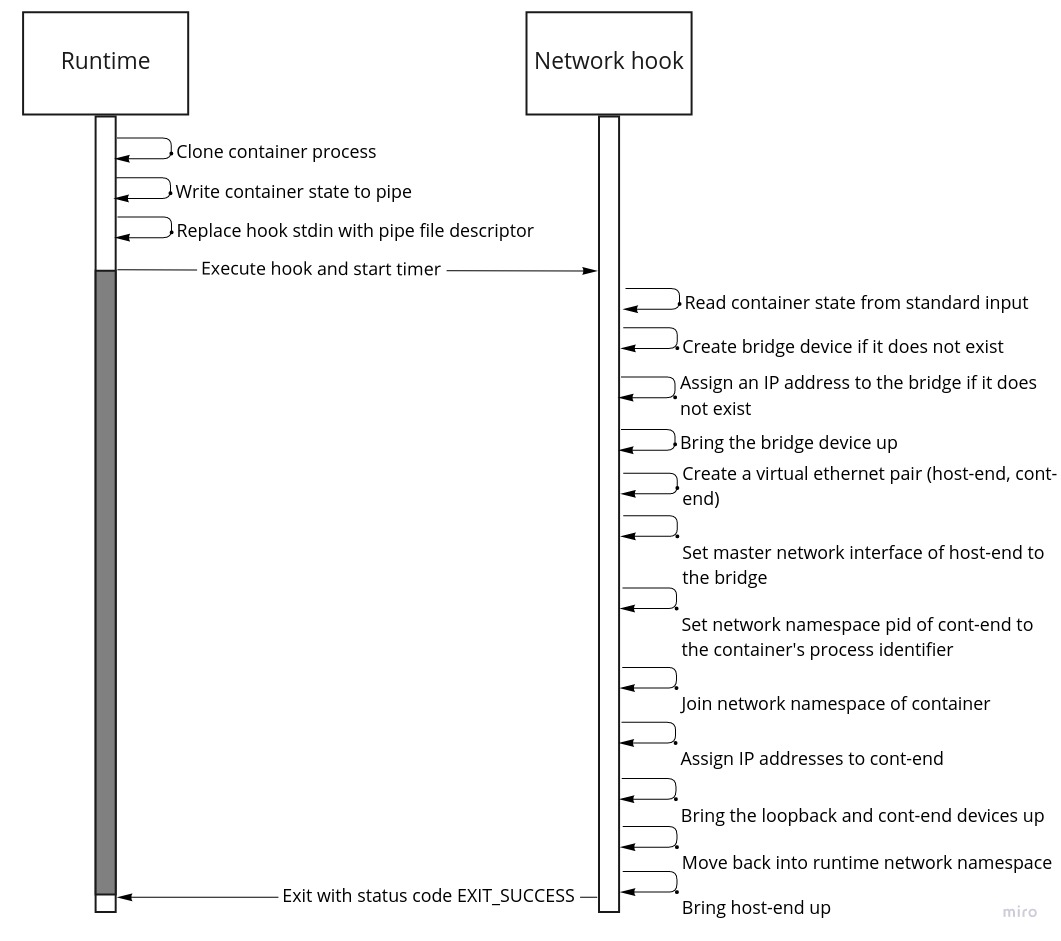
\includegraphics[width=0.7\textwidth]{images/implementation/network-hook-sequence-diagram.jpg}
    \caption{Network hook sequence diagram}
    \label{images:implementation/network-hook-sequence-diagram.jpg}
\end{figure}

The hook's sequence of operations is shown in Figure \ref{images:implementation/network-hook-sequence-diagram.jpg}.
Notice that the hook needs to join the network namespace of the container to setup the network 
addresses of the virtual ethernet cable.
This is done by obtaining a file descriptor to the respective namespace and joining it by 
calling the \verb|setns()| system call. After the configuration is complete, the hook 
returns back to its original namespace by employing the same mechanism. 
The source code of this operation is shown in code snippet \ref{code:implementation/benchmark/network-hook-doer}.

The runtime ensures that the hook program cannot temporally interfere with its execution environment 
by starting a timer before executing it. If the timer expires and the hook has not completed 
its execution, the runtime forcibly kills it. Temporal interference may occur because the runtime 
is required to reap the hook's process identifier. This is done via the \verb|waitpid()| system call,
which suspends the runtime's thread of execution until the hook exits. If the hook does not exit,
it will cause a denial of service by indefinitely blocking the runtime.

The network hook program requires capabilities that the container runtime does not have, namely 
the \verb|CAP_SYS_ADMIN| and \verb|CAP_NET_ADMIN| capabilities. The latter is required 
to configure the network for the container. The former is needed to join the network namespace 
of the container. When the hook program is started, it inherits the capability sets of its parent,
which are insufficient. For this reason, the program is transformed into a \textit{setuid} binary, as shown in 
code snippet \ref{code:implementation/benchmark/network-hook-setuid}.
When executed, the hook inherits the capability sets of the root user without elevating the privileges 
of the runtime.

\begin{lstlisting}[label={code:implementation/benchmark/network-hook-setuid}, style=bash, caption={Building the network hook, changing its ownership and transforming it into a setuid binary by setting the respective permission bit}]
go build -o ./bin/net-hook ./cmd/network/main.go 
sudo chmod u+x ./bin/net-hook
sudo chown root ./bin/net-hook
sudo chmod u+s ./bin/net-hook
\end{lstlisting}

\subsection{Filesystem workload}
The filesystem workload introduced in Section \ref{ch:concept/benchmark/filesystem-workload} was 
implemented with the help of the \verb|fio| program - a tool for simulating input-output workloads 
and sampling performance metrics. \verb|fio| can perform input-output operations directly on 
block devices or on files. In the former case, data is written directly to the device's
addressable memory regions from user space. In the latter case, this is handled by the kernel.
The first option should be handled with care, because \verb|fio| will completely overwrite 
the device's contents. Users can configure the size of the test file with the \verb|--size| option. 
Furthermore, the workloads can be configured to bypass the page cache with the \verb|--direct| option. 
This makes sure that the caching mechanism does not cause any perturbations when assessing 
disk performance. All input-output operations are directed to the underlying device, regardless 
if the file's contents are already present in-memory. The size of the input-output buffers can be 
configured with the \verb|--block-size| option. This option is very important, because it directly 
impacts the latency and throughput results. Larger block sizes typically result in higher 
throughputs, and higher latencies, whereas smaller block sizes lead to lower throughputs and 
lower latencies. Users can also configure the I/O pattern to be employed with the \verb|--mode|
option. When employing mixed input-output operations, the number of reads and writes are equally 
distributed. The available patterns are listed in Table \ref{table:implementation/benchmark/filesystem-workload/io-patterns}.
Fio populates the file with random data, which may cause perturbations during the 
data generation process.
To mitigate this, the program first generates the buffers and reuses 
them. 
This can be bypassed by specifying the \verb|--refill_buffers| option, which refills the 
buffers before every I/O submission. 
Fio provides two modes of submitting parallel I/O operations. 
The most straightforward way to do so is to increase the number of parallel processes via the 
\verb|--numjobs| option. Alternatively, when using an asynchronous I/O engine, the level of 
parallelism can be increased by specifying the \verb|--iodepth| parameter, which regulates 
the number of parallel I/O operations that can be submitted to the kernel via a single 
system call. The I/O engine to use is configured via the \verb|--engine| parameter. It can be set to 
\verb|sync| and \verb|libaio|.

\subsection{Usage \& Reproducibility}
